% IRIS'27 full paper draft. Springer LNCS class until the official template arrives (10 Nov).
\documentclass[runningheads]{llncs}
\usepackage[T1]{fontenc}
\usepackage{graphicx}
\usepackage{amsmath,amssymb}
\usepackage{booktabs}
\usepackage{multirow}
\usepackage{xcolor}
\usepackage{tikz}
\usetikzlibrary{arrows.meta,positioning,fit}
\usepackage[hidelinks]{hyperref}

\newcommand{\focus}{\textsc{focus}}
\newcommand{\fixed}{\textsc{fixed}}

\begin{document}

\title{Anchors That Move Without Collapsing:\\Exclusive-Region Anchor Routing for Vision Transformers}
\titlerunning{Anchors That Move Without Collapsing}

\author{Aadi Gupta}
\authorrunning{A. Gupta}
\institute{Scaler School of Technology, Bengaluru, India\\
\email{aadi.24bcs10167@sst.scaler.com}}

\maketitle

\begin{abstract}
Anchor tokens let a vision transformer exchange global information through a few summary
tokens, but nothing forces different anchors to summarise different things. On one shared
backbone we show that anchors with image-independent queries collapse to a single summary
(pooling-map similarity 0.99--0.999), while an exclusive partition of the patch grid cannot
collapse by construction and is the most accurate pathway in all three seeds on CIFAR-100.
We then propose \emph{focus anchors}: a coarse grid of coverage anchors plus anchors placed
at the peaks of a learned importance map, all sharing one exclusive Voronoi partition, so
anchors move to image content but never pool the same patches. On a cluttered $256^2$
CIFAR-10 canvas trained for 30 epochs, focus anchors beat the fixed partition in 3 of 3
paired seeds (+1.5 points, 95\% CI [0.5, 2.6]) and beat ViTs on downsampled inputs by
4.7--11.8 points on this task and on a Tiny ImageNet canvas. Ablations show that hard exclusive
assignment keeps training stable: its softmax relaxation fails in every seed, also with
Sinkhorn balancing. We also report the
limits: a CNN and PVTv2 are far more accurate in this from-scratch regime, and at $256^2$
our routing is slower than dense attention.
\keywords{Vision transformers \and Anchor tokens \and Token routing \and Representation collapse}
\end{abstract}

% ===========================================================================
\section{Introduction}

Global self-attention in a vision transformer (ViT)~\cite{dosovitskiy2021vit} costs
$O(N^2)$ in the number of patches $N$. At $2048^2$ pixels with $16\times16$ patches,
$N=16{,}384$ and a single dense attention map has $2.7\times10^{8}$ entries. A common remedy
is to route global information through a small set of $A\ll N$ \emph{anchor} (or latent,
inducing, meta, cluster) tokens: patches write into the anchors, the anchors attend to
each other, and the anchors write back~\cite{lee2019settransformer,jaegle2021perceiver,grainger2023paca,jiang2024lemevit,anchorformer2025}.

The bottleneck only helps if the anchors carry \emph{different} information. In our first
anchor model, 32 learned anchors converged to near-identical vectors (pairwise cosine
similarity 0.989--0.995 in every block) and each pooled from almost all 196 patches
(attention entropy 5.272 against a maximum of 5.278): the model had paid for 32 global
summaries and received one. We call this \emph{anchor collapse}.

This paper studies anchor collapse and a way to avoid it while still letting anchors
concentrate on image content. Our contributions are:
\begin{enumerate}
\item A controlled comparison of five anchor pathways on one backbone
(Sec.~\ref{sec:collapse}). Anchors whose queries do not depend on the image collapse almost
completely; image-derived anchors collapse partially; a fixed exclusive partition of the
patch grid cannot collapse and gives the best accuracy in every seed.
\item \emph{Focus anchors} (Sec.~\ref{sec:focus}): coverage anchors on a coarse fixed grid
plus anchors placed at the peaks of a learned importance map, all sharing one exclusive
Voronoi partition. Anchors move to content, yet two anchors can never pool the same patch.
\item A multi-seed evaluation with paired confidence intervals (Sec.~\ref{sec:main}): focus
anchors beat the fixed partition at 10 and 30 epochs and beat ViTs on downsampled inputs on
two datasets; ablations show that hard exclusive assignment is needed for stable training.
\item An explicit account of what does not work (Secs.~\ref{sec:main}--\ref{sec:efficiency}):
a CNN and PVTv2 are far stronger in our from-scratch setting, learned importance does not
select patches for computation better than random, and our routing is slower than dense
attention at moderate resolution; its one efficiency advantage is memory at high resolution.
\end{enumerate}

% ===========================================================================
\section{Related Work}

\paragraph{Latent and anchor bottlenecks.}
Set Transformer inducing points~\cite{lee2019settransformer} and the
Perceiver~\cite{jaegle2021perceiver} cross-attend from a learned latent array to the input,
and TokenLearner~\cite{ryoo2021tokenlearner} learns a few spatial attention maps that pool
tokens. Slot Attention~\cite{locatello2020slot} makes slots compete for inputs with a softmax
over slots. In ViTs, PaCa-ViT~\cite{grainger2023paca} attends from patches to learned
clusters, LeMeViT~\cite{jiang2024lemevit} uses learnable meta tokens, and
AnchorFormer~\cite{anchorformer2025} and Representative Attention~\cite{representative2026}
gather into anchors, let them interact, and distribute back. These methods route tokens
with soft, similarity-based weights, and some normalise the mass each representative
receives to keep all representatives in use. None of them assigns each patch to exactly one
anchor. We show in Sec.~\ref{sec:collapse} that simplified versions of two of them collapse;
we do not reproduce their full models or stabilisers, so this is evidence about the routing
patterns, not about the published methods.

\paragraph{Regional tokens and partitions.}
RegionViT~\cite{chen2022regionvit} attaches one regional token to each fixed window of local
tokens and lets the regional tokens attend globally; our fixed partition is close to this
design, and we do not claim the fixed partition as new. Swin~\cite{liu2021swin} and
PVT~\cite{wang2022pvtv2} reduce attention cost with windows and spatial reduction.
Content-driven groupings, such as super tokens~\cite{huang2023supertoken} and token
clustering~\cite{zeng2022tcformer}, adapt regions to the image but do not keep a fixed
number of exclusive regions with explicit positions.

\paragraph{Learned movement and selection.}
Deformable attention~\cite{xia2022dat} and progressive sampling~\cite{yue2021psvit} learn
where to sample keys or tokens, and recurrent attention~\cite{mnih2014ram} and spatial
transformers~\cite{jaderberg2015stn} learn where to look. For high-resolution inputs under a
memory budget, attention sampling~\cite{katharopoulos2019attsampling} and differentiable or
iterative patch selection~\cite{cordonnier2021dps,bergner2023ips} process only selected
patches. Token pruning and merging~\cite{rao2021dynamicvit,bolya2023tome},
SparseViT~\cite{chen2023sparsevit} and mixture-of-depths~\cite{raposo2024mod} skip
computation for some tokens, and A-ViT~\cite{yin2022avit} and ATS~\cite{fayyaz2022ats}
adapt the number of tokens per image. Our focus anchors move where global summaries are formed, not
which patches exist, and our skipping experiment (Sec.~\ref{sec:skipping}) compares
learned importance against exactly these simpler selection rules.

% ===========================================================================
\section{Method}
\label{sec:method}

\subsection{Local--global--local block}

An image is split into an $S\times S$ grid of $N=S^2$ patches with embeddings
$x_i\in\mathbb{R}^{D}$ and normalised centre coordinates $c_i\in[0,1]^2$. The model keeps
$A$ anchors with features $a_j\in\mathbb{R}^{d}$ ($d<D$) and positions $p_j\in[0,1]^2$.
Each of the $L$ blocks applies (Fig.~\ref{fig:block}):
\begin{enumerate}
\item \textbf{Local attention} within non-overlapping $w\times w$ windows:
$x\leftarrow x+\mathrm{WinAttn}(\mathrm{LN}(x))$.
\item \textbf{Gather}: each anchor pools the patches of its own region $R_j$ (below) with
attention restricted to $R_j$, and the pooled vector is added to $a_j$.
\item \textbf{Global}: anchors attend to each other,
$a\leftarrow a+\mathrm{MHSA}(\mathrm{LN}(a))$; this $A\times A$ attention is the only
long-range interaction.
\item \textbf{Scatter}: each patch reads only its own anchor $a_{r(i)}$ through a sigmoid
gate, $u_i=W_o\,\sigma(q_i^{\top}k_{r(i)}/\sqrt{d_h})\,v_{r(i)}$, and
$x_i\leftarrow x_i+u_i$.
\item \textbf{FFN}: $x\leftarrow x+\mathrm{FFN}(\mathrm{LN}(x))$.
\end{enumerate}
The image is classified from the mean of the final patch tokens.

\begin{figure}[t]
\centering
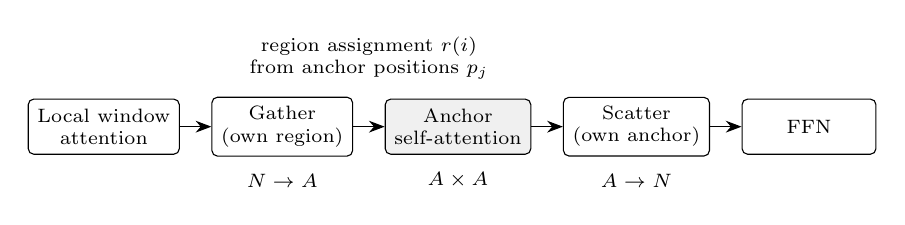
\begin{tikzpicture}[
  box/.style={draw, rounded corners=2pt, minimum height=7mm, minimum width=17mm, font=\scriptsize, align=center},
  arr/.style={-{Stealth[length=2mm]}}, node distance=4mm]
\node[box] (local) {Local window\\attention};
\node[box, right=of local] (gather) {Gather\\(own region)};
\node[box, right=of gather, fill=gray!12] (global) {Anchor\\self-attention};
\node[box, right=of global] (scatter) {Scatter\\(own anchor)};
\node[box, right=of scatter] (ffn) {FFN};
\draw[arr] (local) -- (gather); \draw[arr] (gather) -- (global);
\draw[arr] (global) -- (scatter); \draw[arr] (scatter) -- (ffn);
\node[font=\scriptsize, below=1mm of gather] {$N\to A$};
\node[font=\scriptsize, below=1mm of global] {$A\times A$};
\node[font=\scriptsize, below=1mm of scatter] {$A\to N$};
\node[font=\scriptsize, above=1mm of gather, text width=48mm, align=center, xshift=11mm]
  {region assignment $r(i)$ from anchor positions $p_j$};
\end{tikzpicture}
\caption{One block. Patches communicate locally inside windows and globally only through
their own anchor; the dense $N\times N$ attention of a ViT is replaced by an $A\times A$
attention among anchors.}
\label{fig:block}
\end{figure}

\subsection{Exclusive regions}

Every patch belongs to exactly one anchor: the nearest one,
$r(i)=\arg\min_j\|c_i-p_j\|^2$, which partitions the grid into Voronoi regions
$R_j=\{i: r(i)=j\}$. To let gradients reach the anchor positions, the hard assignment
$h_{ij}=[r(i)=j]$ is used in the forward pass with the gradient of the soft assignment
$s_{ij}=\mathrm{softmax}_j(-\|c_i-p_j\|^2/\tau)$, $\tau=(0.5/\sqrt{A})^2$
(straight-through): $m_{ij}=h_{ij}+s_{ij}-\mathrm{sg}(s_{ij})$.

Anchor $j$ forms queries from $a_j+\phi(p_j)$, with $\phi$ a small MLP of the position, and
pools its region with logits $\ell_{ji}$:
\begin{equation}
w_{ji}=\frac{m_{ij}\exp\!\big(\ell_{ji}-\max_{i'\in R_j}\ell_{ji'}\big)}
{\max\!\big(1,\ \sum_{i'} m_{i'j}\exp(\ell_{ji'}-\max_{i''\in R_j}\ell_{ji''})\big)} .
\label{eq:pool}
\end{equation}
The denominator is clamped at 1 rather than at a small $\epsilon$. A non-empty region always
sums to at least 1, because its best patch contributes $\exp(0)=1$, so the clamp only acts on
\emph{empty} regions. These occur when two moving anchors meet. With an $\epsilon=10^{-9}$
clamp, an empty region produced straight-through gradients of order $10^{9}$ that overflowed
in fp16 and made the first focus models diverge or never learn.

With fixed grid positions $p_j$ this block is \emph{Partition RART} (\fixed). Because the
regions are disjoint, two anchors never pool the same patch: their pooling maps have zero
overlap whatever the weights. This guarantee holds by construction, so zero map similarity
is not by itself evidence that the anchors carry useful, different information; we judge
that by accuracy and by the spread of the pooled content.

\subsection{Focus anchors}
\label{sec:focus}

A fixed partition gives the empty background as many anchors as the object. Focus anchors
let most anchors move to content while keeping the partition exclusive. A linear head gives
each patch a score $z_i=w^{\top}\mathrm{LN}(x)_i$ and importance
$\pi_i=\mathrm{softplus}(z_i)+10^{-3}$. In every block:
\begin{itemize}
\item \textbf{Coverage anchors.} $g^2$ anchors stay on a fixed $g\times g$ grid,
$g=\max(1,\lfloor\sqrt{A/4}\rfloor)$, so that every part of the image keeps a summary
(1 of 4 anchors, or 4 of 16).
\item \textbf{Focus anchors.} The remaining $F=A-g^2$ anchors are placed one at a time by a
soft-argmax over the scores:
$p_k=\sum_i \mathrm{softmax}_i(z_i+b_{ki})\,c_i$. After each placement the scores around
$p_k$ are suppressed, $z_i\leftarrow z_i-\beta\exp(-\|c_i-p_k\|^2/2\sigma_s^2)$, so that the
next anchor goes elsewhere ($\beta=10$, $\sigma_s=1.5$ patches). The term
$b_{ki}=-\|c_i-e_k\|^2/2\sigma_h^2$ is a weak prior towards a spread-out home position $e_k$
($\sigma_h=0.35$), which breaks ties early in training.
\item \textbf{Importance in pooling.} Gather logits are offset by $\log\pi_i$, so anchors
pool important patches more strongly; this also trains the importance head from the
classification loss.
\end{itemize}
All $A$ anchors then share the single Voronoi partition above. Focus anchors can crowd onto
content, which makes their regions small, but they can never share a patch.

As a weaker alternative we also test \textsc{moving} anchors, which take one
importance-weighted Lloyd (k-means) step inside their own region per block, and
\textsc{free} anchors, which have no positions and pool all patches with a softmax
(the RART-16/32 design).

% ===========================================================================
\section{Experiments}

\paragraph{Common setup.}
All anchor models use embedding width $D=384$, depth 6, 6 heads, MLP ratio 3, anchor
width $d=128$ with 4 heads, and patch size 16. All models, baselines included, are trained
from scratch with AdamW (weight decay 0.05), a cosine schedule, batch size 128 and random
horizontal flips, and tested on the full test set. Table~\ref{tab:recipes} lists the
per-experiment settings. Seeds 42, 43 and 44 change the initialisation, data order and
canvas layouts; test canvases use a fixed layout seed. We report paired differences with
95\% $t$-intervals over seeds ($n=3$, so intervals are wide).

\paragraph{Hyperparameter selection.} There is no validation split. Every setting was fixed
in advance except the 30-epoch learning rate: at $3\cdot10^{-4}$ about one in six 30-epoch
runs diverged, and we chose $1.25\cdot10^{-4}$ (the DeiT scaling rule~\cite{touvron2021deit})
after comparing the test accuracy of one run of each at epoch 15. This rate was then used for
every model in that phase; ResNet-18 was also run at $10^{-3}$ and we report its better rate,
also chosen on test accuracy. These choices make the 30-epoch numbers slightly optimistic,
for anchors and baselines alike.

\begin{table}[t]
\centering
\caption{Training settings. All runs: AdamW, weight decay 0.05, cosine schedule, batch 128,
horizontal flip, from scratch. ``Clip'': gradient-norm clipping; ``warmup'': linear, epochs.}
\label{tab:recipes}
\begin{tabular}{lllll}
\toprule
& Collapse & Cluttered, 10 ep. & Cluttered, 30 ep. & Tiny ImageNet \\
\midrule
Data & CIFAR-100, $224^2$ & CIFAR-10 canvas & CIFAR-10 canvas & Tiny IN canvas \\
Train / test & 50k / 10k & 50k / 10k & 50k / 10k & 100k / 10k \\
Epochs & 10 & 10 & 30 & 15 \\
Learning rate & $3\cdot10^{-4}$ & $3\cdot10^{-4}$ & $1.25\cdot10^{-4}$ & $1.25\cdot10^{-4}$ \\
Clip / warmup & -- & --$^{\ast}$ & 1.0 / 2 & 1.0 / 2 \\
Precision & fp16 & fp16 / bf16$^{\dagger}$ & bf16 & bf16 \\
Seeds & 3 & 3 (some 1--2) & 3 & 3 \\
\bottomrule
\end{tabular}

\smallskip
{\scriptsize $^{\ast}$Clip 1.0 / warmup 2 for the stabilised ablations (Table~\ref{tab:ablation},
bottom) and skipping runs marked ``clip''. $^{\dagger}$Table~\ref{tab:moving} and the seed-42
skipping runs in fp16; all later runs in bf16 after fp16 overflow caused divergence.}
\end{table}

\subsection{Anchor collapse across anchor designs}
\label{sec:collapse}

\paragraph{Setup.} CIFAR-100~\cite{krizhevsky2009cifar} at $224^2$ (196 patches), 16
anchors, $7\times7$ local windows. Only the anchor pathway changes:
\textsc{perceiver} (learned queries, softmax over patches, as in RART-16/32),
\textsc{competitive} (the same with a softmax over anchors, as in slot attention),
\textsc{anchorformer}-style (static anchors, softmax over anchors, round trip), a
\textsc{paca}-style pathway (MLP cluster assignment), the fixed exclusive $4\times4$
partition, and a \textsc{dense} pathway that replaces the anchors with global attention
among all patches. The AnchorFormer- and PaCa-style pathways are simplified
reimplementations, not the published models.

\paragraph{Metrics.} For one image and one block, let $P_j\in\Delta^{N-1}$ be anchor $j$'s
pooling distribution over patches and $g_j\in\mathbb{R}^{d}$ the summary it pools. We report
the mean pairwise cosine similarity of the pooling maps and the \emph{spread} of the
summaries,
\begin{equation}
\mathrm{sim}=\frac{1}{A(A-1)}\sum_{j\neq k}\frac{\langle P_j,P_k\rangle}{\|P_j\|\,\|P_k\|},
\qquad
\mathrm{spread}=\frac{\sum_j\|g_j-\bar g\|^2}{\sum_j\|g_j\|^2},\quad \bar g=\frac{1}{A}\sum_j g_j ,
\label{eq:metrics}
\end{equation}
averaged over 1{,}024 test images. Similarity 1 means all anchors pool the same patches;
spread is the share of the summaries' energy that differs between anchors (0 = all anchors
carry the same vector, 1 = summaries with zero mean). Spread measures diversity of the
summaries themselves, so unlike map similarity it is not fixed by the partition.

\begin{table}[t]
\centering
\caption{Anchor collapse on CIFAR-100 at $224^2$ (16 anchors, 10 epochs). Accuracy: mean
$\pm$ std over seeds 42 / 43 / 44 (individual seeds in brackets). Map similarity and spread
are averaged over the 6 blocks, then over seeds.}
\label{tab:collapse}
\begin{tabular}{lccc}
\toprule
Pathway & Test accuracy (\%) & Map similarity & Spread \\
\midrule
\textsc{perceiver} (RART-16) & 40.92 $\pm$ 0.30 {\scriptsize(41.25 / 40.66 / 40.85)} & 0.998 & 0.00 \\
\textsc{competitive} & 42.14 $\pm$ 0.67 {\scriptsize(42.71 / 41.41 / 42.31)} & 0.792 & 0.22 \\
\textsc{anchorformer}-style & 42.52 $\pm$ 0.68 {\scriptsize(42.34 / 43.28 / 41.95)} & 0.990 & 0.06 \\
\textsc{paca}-style & 42.02 $\pm$ 0.07 {\scriptsize(42.08 / 41.94 / 42.04)} & 0.592 & 0.18 \\
\textsc{dense} (no anchors) & 40.93 $\pm$ 0.95 {\scriptsize(42.02 / 40.33 / 40.43)} & -- & -- \\
Fixed partition & \textbf{46.31 $\pm$ 0.56} {\scriptsize(45.68 / 46.48 / 46.77)} & 0.000 & \textbf{0.60} \\
\bottomrule
\end{tabular}
\end{table}

\paragraph{Results.} Table~\ref{tab:collapse} and Fig.~\ref{fig:collapse}. Pathways whose
anchor queries are the same for every image (\textsc{perceiver}, \textsc{anchorformer})
collapse almost completely: map similarity 0.99--0.999 and near-zero spread. Image-derived
anchors (\textsc{competitive}, \textsc{paca}) stay partly diverse, but their summaries grow
more similar with depth. The fixed partition's zero map similarity is guaranteed by
construction; what the experiment shows is that this constraint also gives the highest
spread and the best accuracy, 3.0--5.9 points above every other anchor pathway in each seed
and 5.4 points above the dense pathway on the same backbone. (A standard ViT of the same
width and depth, without local windows, reached 45.44\% in one earlier run.)

\begin{figure}[t]
\centering
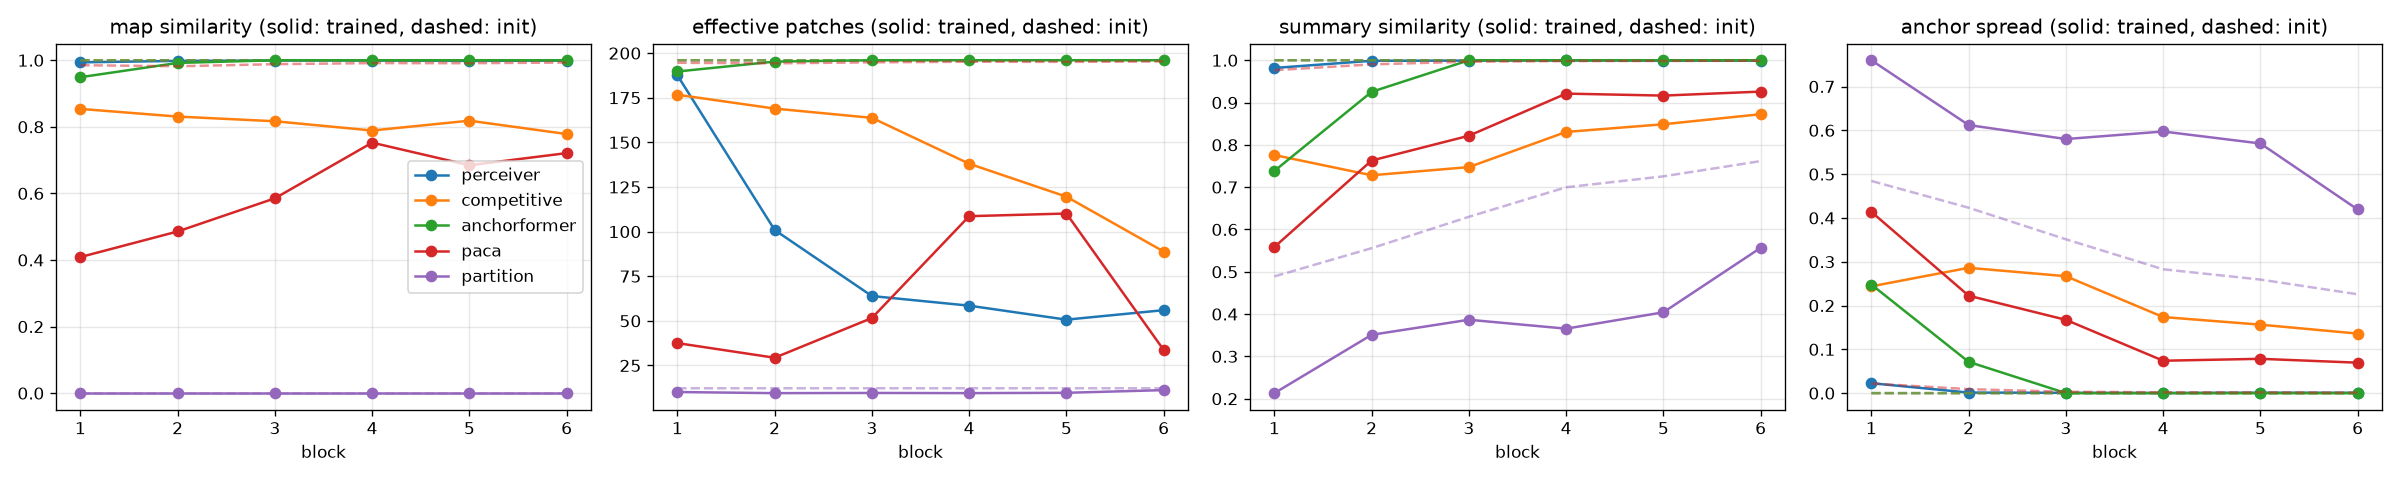
\includegraphics[width=\textwidth]{figures/collapse_metrics_seed42.png}
\caption{Collapse metrics per block (seed 42), trained (solid) and at initialisation
(dashed). The fixed partition (purple) keeps zero map similarity and the highest spread;
image-independent anchors converge to the same summary.}
\label{fig:collapse}
\end{figure}

\subsection{Moving anchors on Cluttered CIFAR-10}
\label{sec:moving}

\paragraph{Task.} CIFAR-10 is too small for anchors to matter, so we build a task in which
most of the image is irrelevant. A $32^2$ CIFAR-10 image is upsampled to $64^2$ and pasted at
a random position on a black $256^2$ canvas ($16\times16$ patches), on top of 8 distractor
fragments (random $16^2$ crops of other training images, upsampled to $32^2$). The object
covers 6.25\% of the canvas. Local windows are $8\times8$ patches.

\begin{table}[t]
\centering
\caption{Cluttered CIFAR-10, 10 epochs. \fixed{} and \focus{}: mean $\pm$ std over seeds
42 / 43 / 44; \textsc{free} and \textsc{moving}: seed 42. ``On object'': share of anchors
whose final-block region contains the object (seed 42). Bottom: paired gaps with 95\% CI.}
\label{tab:moving}
\begin{tabular}{lcccc}
\toprule
& \multicolumn{2}{c}{Test accuracy (\%)} & Map & On object \\
Model & 4 anchors & 16 anchors & similarity & (4 / 16) \\
\midrule
\textsc{free} & 47.00 & 47.82 & 0.998 & -- \\
\textsc{moving} & 47.61 & 48.64 & 0.000 & 0.33 / 0.20 \\
\fixed & 46.04 $\pm$ 0.94 & 46.71 $\pm$ 1.72 & 0.000 & 0.39 / 0.19 \\
\focus & \textbf{47.52 $\pm$ 1.11} & \textbf{49.84 $\pm$ 0.26} & 0.000 & \textbf{0.57} / 0.24 \\
\bottomrule
\end{tabular}

\vspace{2mm}
\begin{tabular}{lccccc}
\toprule
Paired gap \focus{} $-$ \fixed{} & seed 42 & seed 43 & seed 44 & mean & 95\% CI \\
\midrule
4 anchors & +1.71 & +1.23 & +1.51 & +1.48 & [+0.88, +2.08] \\
16 anchors & +1.53 & +2.90 & +4.96 & +3.13 & [$-$1.16, +7.42] \\
\bottomrule
\end{tabular}
\end{table}

\paragraph{Results.} Table~\ref{tab:moving}. Focus anchors beat the fixed partition in all
six paired runs, by 1.2--1.7 points with 4 anchors and 1.5--5.0 points with 16; with 16
anchors the gap varies enough across seeds that its interval still includes zero, and we
return to it at 30 epochs (Sec.~\ref{sec:main}). With 16 anchors, focus accuracy varies far
less across seeds (49.6--50.1\% against 44.8--48.1\%). With 4 anchors the share of anchors
whose region contains the object rises from 0.44 in the first block to 0.57 in the last;
for \fixed{} it stays at 0.39.

Two baselines explain why the design needs both parts. \textsc{free} anchors collapse (map
similarity 0.998), but onto the object, which does no harm on a single-object task, so
\textsc{free} stays level with \fixed. \textsc{moving} anchors find the object in their
importance map (4--9$\times$ more importance per patch than background) yet move only about
one patch, because a Lloyd step keeps each anchor inside its own region: a coverage rule
cannot concentrate anchors. Focus anchors are placed globally, then partitioned.

Fig.~\ref{fig:anchors} shows that focus anchors gather on \emph{all} image content, the
object and the distractors, and leave the empty background to a few large coverage
regions. The importance map learns ``where there is content'', not ``where the object
is'', which is what we would expect when the distractors are real image fragments. We
therefore describe focus anchors as moving to content, not to the object.

\begin{figure}[t]
\centering
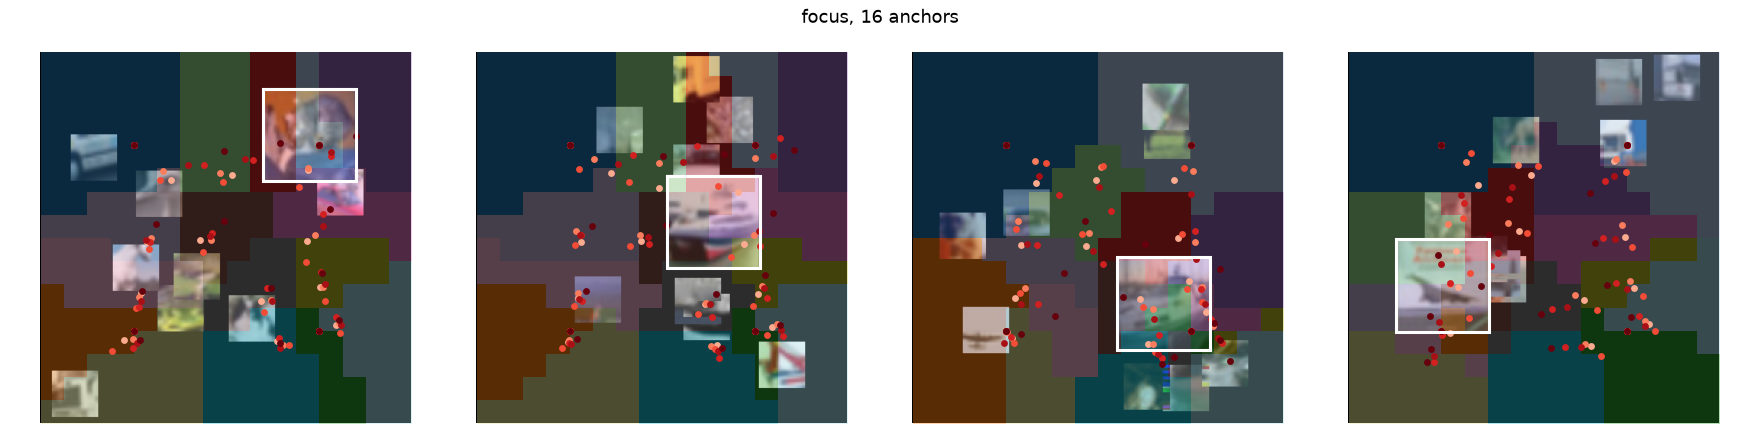
\includegraphics[width=\textwidth]{figures/focus_A16_seed42.png}
\caption{Final-block regions (colours) and anchor positions in each block (dots, darker =
later) of \focus{} with 16 anchors on four test canvases; the white box is the object. Focus
anchors gather on image content and leave empty background to large coverage regions.}
\label{fig:anchors}
\end{figure}

\subsection{Main comparison}
\label{sec:main}

\paragraph{Setup.} We compare \focus{} and \fixed{} with a dense ViT of the same width and
depth (global attention in every block, no local windows) on the full $256^2$ canvas, and
with the same ViT on an area-downsampled $128^2$ input (patch 16) or $64^2$ input (patch 8),
which cost about a quarter of the FLOPs. As stronger references from outside our model family
we add PVTv2-B0~\cite{wang2022pvtv2} and ResNet-18~\cite{he2016resnet} (\texttt{timm}, no
pretraining). Besides Cluttered CIFAR-10 we use a \emph{Tiny ImageNet canvas}: a
$64^2$ Tiny ImageNet~\cite{le2015tinyimagenet} image (200 classes) pasted without resizing
on the $256^2$ canvas among 8 native $32^2$ crops of other images, with the 10k validation
images as the test set. Here the object carries real detail at full resolution, and
downsampling the canvas to $128^2$ halves it.

\begin{table}[t]
\centering
\caption{Main comparison, test accuracy (\%), mean $\pm$ std over 3 seeds. GFLOPs per image
include attention. ``Cluttered'': Cluttered CIFAR-10; ``Tiny IN'': Tiny ImageNet canvas.
\focus{}/\fixed{} at 10 epochs from Table~\ref{tab:moving}. ResNet-18: learning rate $10^{-3}$
(at $1.25\cdot10^{-4}$: 74.29 and 20.16).}
\label{tab:main}
\begin{tabular}{lrrccc}
\toprule
& & & \multicolumn{2}{c}{Cluttered} & Tiny IN \\
Model & Params & GFLOPs & 10 ep. & 30 ep. & 15 ep. \\
\midrule
\focus-16 & 11.4M & 5.49 & 49.84 $\pm$ 0.26 & \textbf{66.82 $\pm$ 0.66} & 17.68 $\pm$ 0.33 \\
\focus-4 & 11.4M & 5.45 & 47.52 $\pm$ 1.11 & 64.67 $\pm$ 0.26 & -- \\
\fixed-16 & 11.4M & 5.49 & 46.71 $\pm$ 1.72 & 65.29 $\pm$ 0.94 & 16.73 $\pm$ 0.46 \\
ViT, $256^2$ & 9.3M & 5.28 & 46.74 $\pm$ 0.42 & 61.99 $\pm$ 0.54 & \textbf{18.25 $\pm$ 0.33} \\
ViT, $128^2$ & 9.2M & 1.21 & 43.20 $\pm$ 0.22 & 55.05 $\pm$ 0.26 & 12.49 $\pm$ 0.28 \\
ViT, $64^2$, patch 8 & 9.0M & 1.18 & 42.39 $\pm$ 0.41 & -- & 13.01 $\pm$ 0.39 \\
\midrule
PVTv2-B0 & 3.4M & 1.51 & 71.83 $\pm$ 0.30 & 75.07 $\pm$ 0.25 & -- \\
ResNet-18 & 11.2M & 4.74 & -- & 86.11 $\pm$ 0.26 & 37.07 $\pm$ 0.28 \\
\bottomrule
\end{tabular}

\vspace{2mm}
\begin{tabular}{lcc}
\toprule
Paired gap, mean [95\% CI] & Cluttered, 30 ep. & Tiny IN, 15 ep. \\
\midrule
\focus-16 $-$ \fixed-16 & +1.54 [+0.53, +2.55] & +0.95 [$-$0.93, +2.83] \\
\focus-16 $-$ ViT $256^2$ & +4.83 [+3.86, +5.80] & $-$0.58 [$-$2.11, +0.95] \\
\fixed-16 $-$ ViT $256^2$ & +3.29 [+1.32, +5.27] & $-$1.53 [$-$1.89, $-$1.16] \\
\focus-16 $-$ ViT $128^2$ & +11.77 [+9.73, +13.82] & +5.19 [+4.43, +5.95] \\
\bottomrule
\end{tabular}
\end{table}

\begin{figure}[t]
\centering
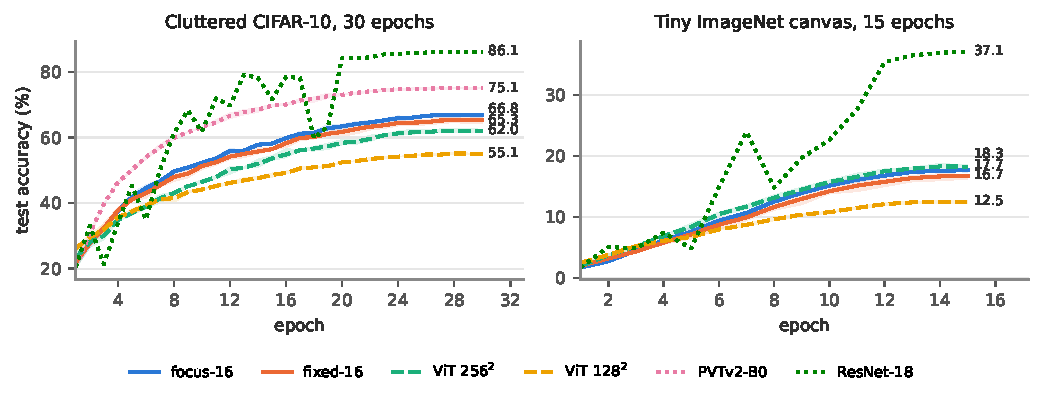
\includegraphics[width=\textwidth]{figures/curves.pdf}
\caption{Test accuracy during training, mean over 3 seeds (band: min--max; omitted for
ResNet-18, whose per-epoch test accuracy fluctuates strongly). Anchor models solid,
baselines dashed or dotted. PVTv2-B0 was not run on Tiny ImageNet.}
\label{fig:curves}
\end{figure}

\paragraph{Results.} Table~\ref{tab:main} and Fig.~\ref{fig:curves}.
\emph{Focus versus fixed.} With 30 epochs, focus anchors beat the fixed partition in all three
seeds (+1.1 to +1.8 points), and the interval excludes zero. On the Tiny ImageNet canvas
focus anchors are ahead in all three seeds as well (+0.4 to +1.8), but the interval includes
zero. Four focus anchors do not match sixteen fixed ones ($-$0.6 points).
\emph{Against downsampling.} Focus anchors beat a ViT on a $128^2$ or $64^2$ input by
4.7--11.8 points on both datasets, the fixed partition by 3.5--10.2. On Cluttered CIFAR-10 the $128^2$ input keeps the object at its
native $32^2$ resolution, so the loss there comes from coarser tokens (the object spans only
$2\times2$ patches), not from lost pixels; on the Tiny ImageNet canvas the object loses half
its resolution as well.
\emph{Against dense attention at full resolution.} On Cluttered CIFAR-10 both anchor models
beat the dense ViT at matched FLOPs (+4.8 and +3.3 points). This baseline has no local
windows, so part of this gap is the locality bias of the windowed blocks rather than the
anchors; the effect of anchor movement alone is the \focus{}$-$\fixed{} gap. On the Tiny
ImageNet canvas the dense ViT is level with focus anchors and ahead of the fixed partition.
\emph{Against established architectures.} PVTv2-B0 and ResNet-18 are far more accurate:
75.1\% and 86.1\% against 66.8\% on Cluttered CIFAR-10, and ResNet-18 reaches 37.1\% against
17.7\% on the Tiny ImageNet canvas. Trained from scratch on 50k--100k images for 15--30 epochs,
the convolutional bias of these models matters more than how a plain transformer routes
global information~\cite{dosovitskiy2021vit,touvron2021deit}. Our claims are therefore about
anchor routing \emph{within} transformers of this kind, not about the best model for these tasks.

\subsection{Ablations of focus anchors}
\label{sec:ablation}

\begin{table}[t]
\centering
\caption{Ablations on Cluttered CIFAR-10 (16 anchors, 10 epochs, seeds 42 / 43 / 44).
Top: recipe of Table~\ref{tab:moving}; ``diverged'': gradient norm $>10^{5}$, training lost.
Bottom: with gradient clipping 1.0 and 2-epoch warmup.}
\label{tab:ablation}
\begin{tabular}{lcl}
\toprule
Variant & Test accuracy (\%) & Note \\
\midrule
\focus-16 (full) & 49.84 $\pm$ 0.26 & \\
No coverage grid (16 focus anchors) & 49.63 $\pm$ 0.28 & \\
$3\times3$ coverage grid (7 focus anchors) & 49.40 $\pm$ 0.78 & \\
No home prior & 47.23 $\pm$ 1.17 & $-$2.6 points \\
No suppression & 49.34 / 13.25 / 48.89 & diverged in seed 43 \\
Soft instead of hard assignment & 14.34 / 36.17 / 10.00 & diverged in seeds 42, 44 \\
\midrule
\focus-16 (full), clip & 53.78 $\pm$ 0.09 & \\
No suppression, clip & 53.57 $\pm$ 0.43 & $-$0.21 [$-$1.51, +1.08] \\
Soft assignment, clip & 10.00 / 10.00 / 10.00 & diverged in all seeds \\
Soft + Sinkhorn balancing, clip & 9.98 / 10.00 / 12.44 & diverged in all seeds \\
\bottomrule
\end{tabular}
\end{table}

Table~\ref{tab:ablation}. The coverage grid makes no measurable difference: without it the
focus anchors still cover the canvas, and a larger grid neither helps nor hurts. The home
prior matters ($-$2.6 points without it): early in training it keeps focus anchors spread
out until the importance map has learned something. Suppression does not change accuracy
once training is stabilised, but without it one of three runs diverged under the basic
recipe; with all anchors free to land on the same peak, regions can empty and refill
abruptly. The clearest result is soft assignment: replacing the hard Voronoi partition by
its softmax relaxation diverged or stalled in every run, and still diverged in all three
seeds with clipping and warmup (gradient norms reaching $10^{14}$ at epoch 6). Balancing does
not fix it. With three log-domain Sinkhorn iterations after the softmax, so that every anchor
receives the same total mass as in balanced soft routing, the runs learned for two to five
epochs (peaks of 37.5, 26.5 and 39.0\%) and then diverged in all three seeds, with gradient
norms of $10^{11}$--$10^{15}$ despite clipping. Hard exclusive assignment is what makes moving
anchors trainable here.

\begin{table}[t]
\centering
\caption{Sensitivity of focus placement (Cluttered CIFAR-10, 16 anchors, 10 epochs, clip 1.0,
warmup 2, seed 42). One parameter changed at a time from the defaults $\beta=10$,
$\sigma_s=1.5$ patches, $\sigma_h=0.35$.}
\label{tab:sensitivity}
\begin{tabular}{lcc}
\toprule
Setting & Test accuracy (\%) & $\Delta$ \\
\midrule
Defaults & 53.68 & \\
$\beta=3$ & 53.98 & +0.30 \\
$\beta=30$ & 49.33 & $-$4.35 \\
$\sigma_s=0.75$ & 53.59 & $-$0.09 \\
$\sigma_s=3$ & 21.88 & $-$31.80 \\
$\sigma_h=0.15$ & 52.90 & $-$0.78 \\
$\sigma_h=1.0$ & 52.26 & $-$1.42 \\
\bottomrule
\end{tabular}
\end{table}

Table~\ref{tab:sensitivity} varies the placement hyperparameters one at a time, with one seed
each, so differences below about one point are within seed noise
(Table~\ref{tab:ablation}). Weaker or narrower suppression and a narrower or wider home prior
stay within 1.5 points of the defaults. Placement breaks when suppression is too strong or too
wide: $\beta=30$ costs 4.4 points, and with $\sigma_s=3$ patches training stalls near 20\% for
all ten epochs. A suppression bump three patches wide covers much of the $16\times16$ grid, so
later focus anchors are pushed away from the content the importance map has found.

\subsection{Skipping per-patch computation}
\label{sec:skipping}

Anchors are a negligible share of the compute: \textsc{free}, \fixed{} and \focus{} with 16
anchors all cost about 5.31 GFLOPs per image (linear layers), so savings have to come from
per-patch work. From block 3 on, only a fraction of patches go through the FFN, the most
expensive part of each block. The other patches skip it, but they have already received
their anchor's global update. We compare three ways of choosing the kept patches: the
learned importance $\pi_i$ (trained through a straight-through gate), uniform random, and the
token $L_2$ norm, as in SparseViT~\cite{chen2023sparsevit}.

\begin{table}[t]
\centering
\caption{FFN skipping on Cluttered CIFAR-10 (\focus-16, 10 epochs). FFN of blocks 3--6 applied
to the kept share of patches. GFLOPs count linear layers. Gate: $\pi/\mathrm{sg}(\pi)$
(``ratio'') or $1+\pi-\mathrm{sg}(\pi)$ (``bounded'').}
\label{tab:skip}
\begin{tabular}{llccc}
\toprule
Kept & Chosen by & Seeds & Test acc. (\%) & GFLOPs \\
\midrule
100\% & -- & 42 & 49.63 & 5.31 \\
25\% & learned importance, ratio gate & 42 & 49.25 & 3.96 \\
25\% & random & 42 / 43 / 44 & 50.49 / 50.15 / 46.76 & 3.96 \\
25\% & token norm & 42 / 43 / 44 & 50.87 / 52.16 / 50.82 & 3.96 \\
50\% & learned importance, ratio gate & 42 & 38.25 & 4.41 \\
25\% & learned importance, bounded gate & 42 / 43 / 44 & 15.67 / 28.50 / 14.27 & 3.96 \\
50\% & learned importance, bounded gate & 42 & 15.09 & 4.41 \\
\midrule
100\%, clip & -- & 3 & 53.78 $\pm$ 0.09 & 5.31 \\
25\%, clip & random & 3 & 53.40 $\pm$ 0.35 & 3.96 \\
\bottomrule
\end{tabular}
\end{table}

Table~\ref{tab:skip}: skipping the FFN for 75\% of patches in the last four blocks removes
25\% of the linear-layer FLOPs at little or no cost in accuracy. With the stabilised recipe,
random skipping is within 0.4 points of the full model ($-$0.38, 95\% CI [$-$1.48, +0.71]).
The learned importance map, however, does not choose better than random or token-norm
selection, and training through it is fragile. With the ratio gate, keeping 50\% by
importance destabilised training (38.25\%); we attributed this to the gate's gradient
$1/\pi$, which is large for kept patches of low importance. The bounded gate
$1+\pi-\mathrm{sg}(\pi)$ avoids that term but diverged in every run, at 25\% and at 50\%,
and also with clipping and warmup (two further runs, stopped at epoch 5 near 20\%). On
this canvas a 25\% budget covers nearly all image content, so every rule keeps the object;
a smaller budget or a smaller object may separate the rules.

\subsection{Efficiency}
\label{sec:efficiency}

\begin{table}[t]
\centering
\caption{Cost at $256^2$ on one A100 (bf16, untrained, measured alone). Training step: forward
and backward, batch 128.}
\label{tab:cost}
\begin{tabular}{lrrrrr}
\toprule
Model & GFLOPs & Train step & Train memory & Inference & Inf.\ memory \\
\midrule
\focus-16 & 5.49 & 99.3 ms & 4.53 GB & 5{,}259 img/s & 767 MB \\
\focus-16, keep 25\% & 4.13 & 93.0 ms & 4.05 GB & 5{,}248 img/s & 767 MB \\
\focus-4 & 5.45 & 70.8 ms & 4.24 GB & 6{,}207 img/s & 765 MB \\
\fixed-16 & 5.49 & 60.7 ms & 4.31 GB & 6{,}408 img/s & 766 MB \\
ViT, $256^2$ & 5.28 & 32.4 ms & 3.11 GB & 11{,}176 img/s & 728 MB \\
ViT, $128^2$ & 1.21 & 20.6 ms & 1.17 GB & 39{,}339 img/s & 536 MB \\
PVTv2-B0 & 1.51 & 52.4 ms & 4.94 GB & 6{,}310 img/s & 1{,}174 MB \\
\bottomrule
\end{tabular}
\end{table}

\paragraph{At $256^2$ anchors cost more than dense attention.} Table~\ref{tab:cost}. With 256
patches, dense attention is cheap, and our routing (masked gather and scatter, plus one
sequential soft-argmax per focus anchor) is not fused into efficient kernels. The fixed
partition takes 1.9$\times$ and focus anchors 3.1$\times$ the training-step time of the dense
ViT at the same FLOPs, and both use more training memory. The sequential placement loop
accounts for the gap between focus and fixed anchors: it adds about 3--4 ms per focus anchor
per training step (99.3 against 60.7 ms with 12 focus anchors, 70.8 against 59.5 ms with 3). FFN skipping lowers FLOPs but
barely changes wall-clock time, because the gather and scatter of kept patches is not fused.

\begin{table}[t]
\centering
\caption{Resolution scaling of the fixed partition: inference on a Tesla T4 (batch 2; batch 1
at $2048^2$), untrained models, one anchor per $4\times4$ block of patches. Bottom: $2048^2$,
batch 1, against efficient transformers from \texttt{timm}.}
\label{tab:scaling}
\begin{tabular}{rcccc}
\toprule
Resolution & RART latency & ViT latency & RART memory & ViT memory \\
\midrule
$224^2$ & 35.4 ms & 5.5 ms & 62 MB & 61 MB \\
$512^2$ & 119.4 ms & 28.5 ms & 103 MB & 180 MB \\
$1024^2$ & 454.9 ms & 261.2 ms & 252 MB & 1{,}704 MB \\
$1280^2$ & 717.6 ms & 632.8 ms & 365 MB & 3{,}984 MB \\
$1536^2$ & 1{,}022.9 ms & 1{,}251.9 ms & 506 MB & 8{,}091 MB \\
$2048^2$ & 1{,}641.8 ms & 2{,}125.2 ms & 463 MB & 12{,}582 MB \\
\bottomrule
\end{tabular}

\vspace{2mm}
\begin{tabular}{lccc}
\toprule
Model ($2048^2$, batch 1) & Parameters & Latency & Peak memory \\
\midrule
Partition RART & 17.62M & 1{,}641.8 ms & 463 MB \\
Dense ViT & 17.27M & 2{,}125.2 ms & 12{,}582 MB \\
PVTv2-B1~\cite{wang2022pvtv2} & 13.55M & 804.8 ms & 1{,}901 MB \\
EfficientViT-B2~\cite{cai2023efficientvit} & 22.03M & 207.2 ms & 1{,}007 MB \\
\bottomrule
\end{tabular}
\end{table}

\paragraph{At high resolution the fixed partition saves memory, not time.}
Table~\ref{tab:scaling}. With one anchor per $4\times4$ patches, the fixed partition's
inference memory stays below 0.6 GB up to $2048^2$, where the dense ViT needs 12.6 GB
(27$\times$ more); it overtakes dense attention in latency between $1280^2$ and $1536^2$. It
is \emph{not} faster than established efficient transformers: PVTv2-B1 is about 2$\times$ and
EfficientViT-B2 about 8$\times$ faster. We have not measured focus anchors at these
resolutions; their sequential placement loop grows with the number of focus anchors.

% ===========================================================================
\section{Limitations}

Our tasks are small and synthetic: CIFAR-100 at $224^2$ and two canvases built from
low-resolution images. They isolate the mechanism, but they do not show that focus anchors
help on real high-resolution data, such as traffic-sign recognition~\cite{larsson2011sts},
where a small object carries detail that downsampling destroys. All models are trained from
scratch for 10--30 epochs, are far from convergence (absolute accuracy on the Tiny ImageNet
canvas is below 20\% for every transformer), and are clearly beaten by a CNN and by PVTv2.
Three seeds give wide intervals, and several skipping and baseline rows use one or two seeds.
There is no validation split, and the 30-epoch learning rate was chosen on test accuracy. The
dense ViT baseline has no local windows, so it does not isolate the anchors from locality. We
compare with simplified reimplementations of AnchorFormer- and PaCa-style routing, not with
the published models and their stabilisers; our Sinkhorn test balances anchor mass but does
not add their other stabilisers. The placement hyperparameters were set once; the sensitivity
sweep uses one seed per setting and shows a failure range ($\sigma_s=3$) rather than a tuned
optimum. The
learned importance map marks content in general rather than the class object, and it does not
beat simple rules for choosing which patches to compute. Finally, our implementation is not
optimised; at moderate resolution it is slower than dense attention.

\section{Conclusion}

Anchor bottlenecks only pay off if the anchors stay different. We found that anchors with
image-independent queries collapse to a single summary, and that an exclusive partition of
the patch grid prevents collapse by construction and gives the most accurate anchor pathway.
Focus anchors keep that guarantee while letting most anchors move to image content: they beat
the fixed partition in every paired run on Cluttered CIFAR-10, significantly so at 30
epochs, and beat ViTs on downsampled inputs by 4.7--11.8 points on two datasets. In our setup, hard
exclusive assignment is what makes moving anchors trainable: its soft relaxation does not
train, with or without Sinkhorn balancing. The gains are modest and sit
well below convolutional and hierarchical models in our from-scratch setting, and the
efficiency benefit is limited to memory at high resolution. The next step is a real
high-resolution task with pretrained backbones, where a model that does not have to
downsample the image should show its advantage. Further directions are letting each patch
read a few neighbouring anchors instead of one, a balancing loss against empty regions in
place of the clamp, and weak supervision that steers focus anchors towards the class object
rather than all content.

\paragraph{Code and data availability.} Code, per-run logs and result files for every
experiment: \url{https://github.com/ARRY7686/Partitioned-Residual-Anchor-Routing-Transformer}.

\bibliographystyle{splncs04}
\bibliography{refs}

\end{document}
